\documentclass[aps,prapplied,reprint,superscriptaddress,nofootinbib,floatfix]{revtex4-2}

% Supplemental Material of nvision_paper.tex (main.tex on Overleaf). Compiled as its own document; its labels start
% sm:, and it refers to equations and sections of the main text through xr-hyper.
\usepackage{amsmath,amssymb}
\setcounter{secnumdepth}{3}
\usepackage{xcolor}
\usepackage{graphicx}
\graphicspath{{figures/}}
\usepackage{xr-hyper}
% The main document is nvision_paper.tex locally and main.tex on Overleaf.
\IfFileExists{main.tex}{\externaldocument{main}}{\externaldocument{nvision_paper}}
\usepackage{hyperref}
\hypersetup{colorlinks=true, linkcolor=blue!50!black, citecolor=blue!50!black, urlcolor=blue!60!black}

\newcommand{\code}[1]{\texttt{#1}}
\newcommand{\tbd}[1]{\textcolor{red}{[#1]}}
\newcommand{\SM}[1]{Sec.~\ref{#1}}

% Supplemental numbering: Sec. S1, Eq. (S1), Fig. S1.
\renewcommand{\thesection}{S\arabic{section}}
\renewcommand{\theequation}{S\arabic{equation}}
\renewcommand{\thefigure}{S\arabic{figure}}
\renewcommand{\thetable}{S\arabic{table}}

\begin{document}

\title{Supplemental Material: Following the Information Bound from a Search-Window Prior with Sequential Bayesian
Experiment Design in Nitrogen-Vacancy Magnetometry}

\author{\tbd{Authors}}
\affiliation{\tbd{Affiliation}}

\maketitle

Equations, sections and figures without the prefix S refer to the main text.

% =====================================================================
\section{ODMR physics and line shapes}
\label{sm:odmr}
% =====================================================================

This section gives the physics behind the line model of Sec.~\ref{sec:model} of the main text: the optical
readout of the N-V spin, the Rabi response that sets the CW and pulsed line shapes, the hyperfine structure and the
second transition that Eq.~\eqref{eq:signal} leaves out, and the derivation of the line shapes with the laser
treated as two rates rather than a reset, the broadening by the spin bath, and the pulsed readout.

\subsection{Optical readout}

The negatively charged N-V center is described by five levels
\cite{manson2006,doherty2013nv} (Fig.~\ref{fig:levels}): the spin-triplet ground state $^3A_2$, split into
$|0\rangle_g$ and $|\pm1\rangle_g$ by the spin projection $m_s$ on the N-V axis; the spin-triplet excited state
$^3E$, with $|0\rangle_e$ and $|\pm1\rangle_e$; and a metastable spin singlet $|s\rangle$ that stands for the
singlet manifold. Green light drives the spin-conserving optical transitions $|m_s\rangle_g\to|m_s\rangle_e$, which
decay back by emitting red photoluminescence (PL). From $|\pm1\rangle_e$, however, the intersystem crossing to the
singlet is much faster than from $|0\rangle_e$, and the singlet decays preferentially to $|0\rangle_g$.
% The singlet -> |g,0> branching ratio is still debated: ~50-70 % (Robledo et al. 2011; Tetienne et al. 2012)
% vs ~90 % (Wirtitsch et al.), as summarized in arXiv:2511.19583. Not needed here: only the net pumping into
% m_s = 0 enters, through the rate Gamma_p below. Verify the primary sources before quoting a number.
Two
consequences follow. Under continuous illumination the spin is pumped into $m_s=0$; and a center in $m_s=\pm1$
spends part of its optical cycles in the dark singlet, so it emits less PL than one in $m_s=0$. The spin state can
therefore be prepared and read out optically.
\begin{figure}[t]
\centering
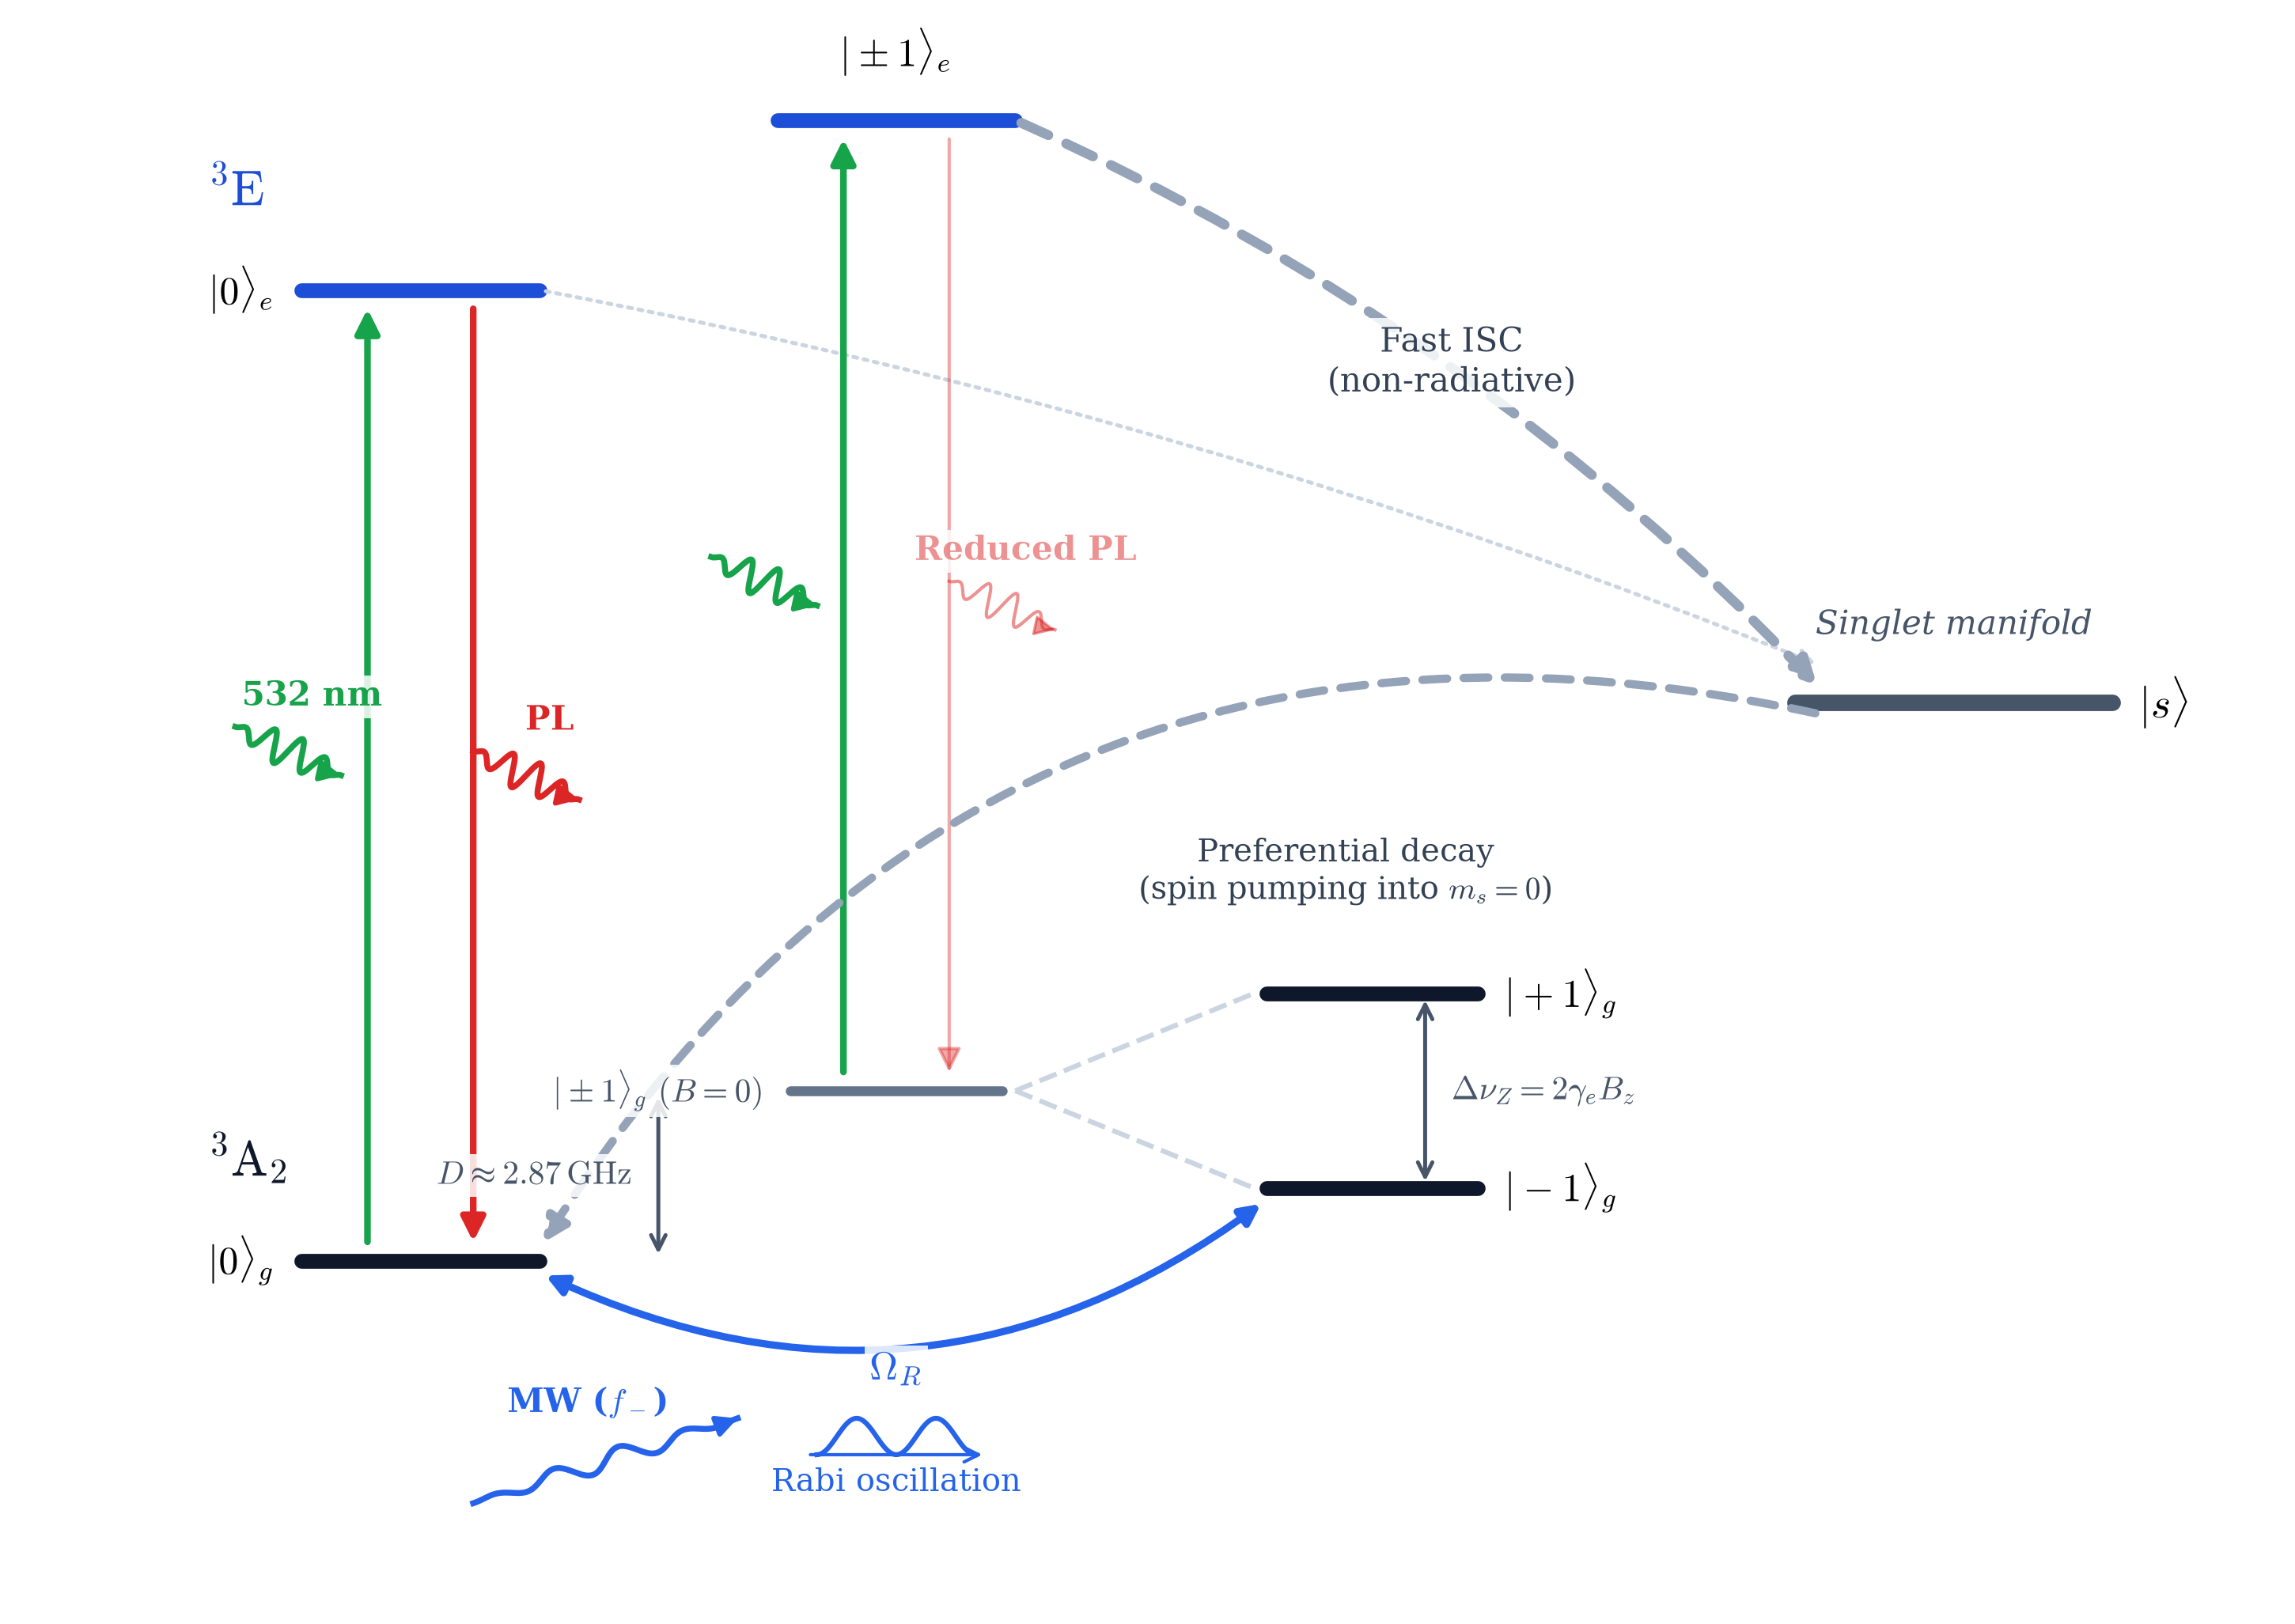
\includegraphics[width=\linewidth]{nv_5level_diagram}
\caption{Five-level model of the N-V center \cite{manson2006,doherty2013nv}. \tbd{Caption to follow the figure.}}
\label{fig:levels}
\end{figure}

The two transitions $f_\pm$ share the state $|0\rangle_g$ but lie $2\delta_Z$ apart. When this separation is large
compared with the linewidth, a drive near $f_-$ is far off resonance with $f_+$ and couples only $|0\rangle_g$ and
$|-1\rangle_g$. The excited state and the singlet then enter only through the rates at which the laser repolarizes
the spin and destroys its coherence \cite{dreau2011}, so the spin reduces to a driven two-level system
$\{m_s=0,m_s=-1\}$.

\subsection{Rabi response and the two ODMR modes}

Let the drive have detuning $\Delta=f-f_-$ from the transition and Rabi frequency $\Omega$, the rate in Hz at which
the population oscillates on resonance. Off resonance the spin oscillates faster but less deeply, at the
generalized Rabi frequency
\begin{equation*}
  \Omega_{\rm gen}=\sqrt{\Omega^2+\Delta^2}.
\end{equation*}
Starting from $m_s=0$, the probability of finding the spin in $m_s=-1$ after a drive of duration $t$ is
\begin{equation}
  P_{-1}(\Delta,t)=\frac{\Omega^2}{\Omega_{\rm gen}^2}\,\sin^2\!\big(\pi\Omega_{\rm gen} t\big),
  \label{eq:rabi}
\end{equation}
and $P_0=1-P_{-1}$ is the probability of finding it still in $m_s=0$. The prefactor is the depth of the
oscillation, the sine its time dependence. Since $m_s=-1$ is the darker state, the PL dip is proportional to
$P_{-1}$. How the drive is applied sets the line shape.
\begin{figure}[t]
\centering
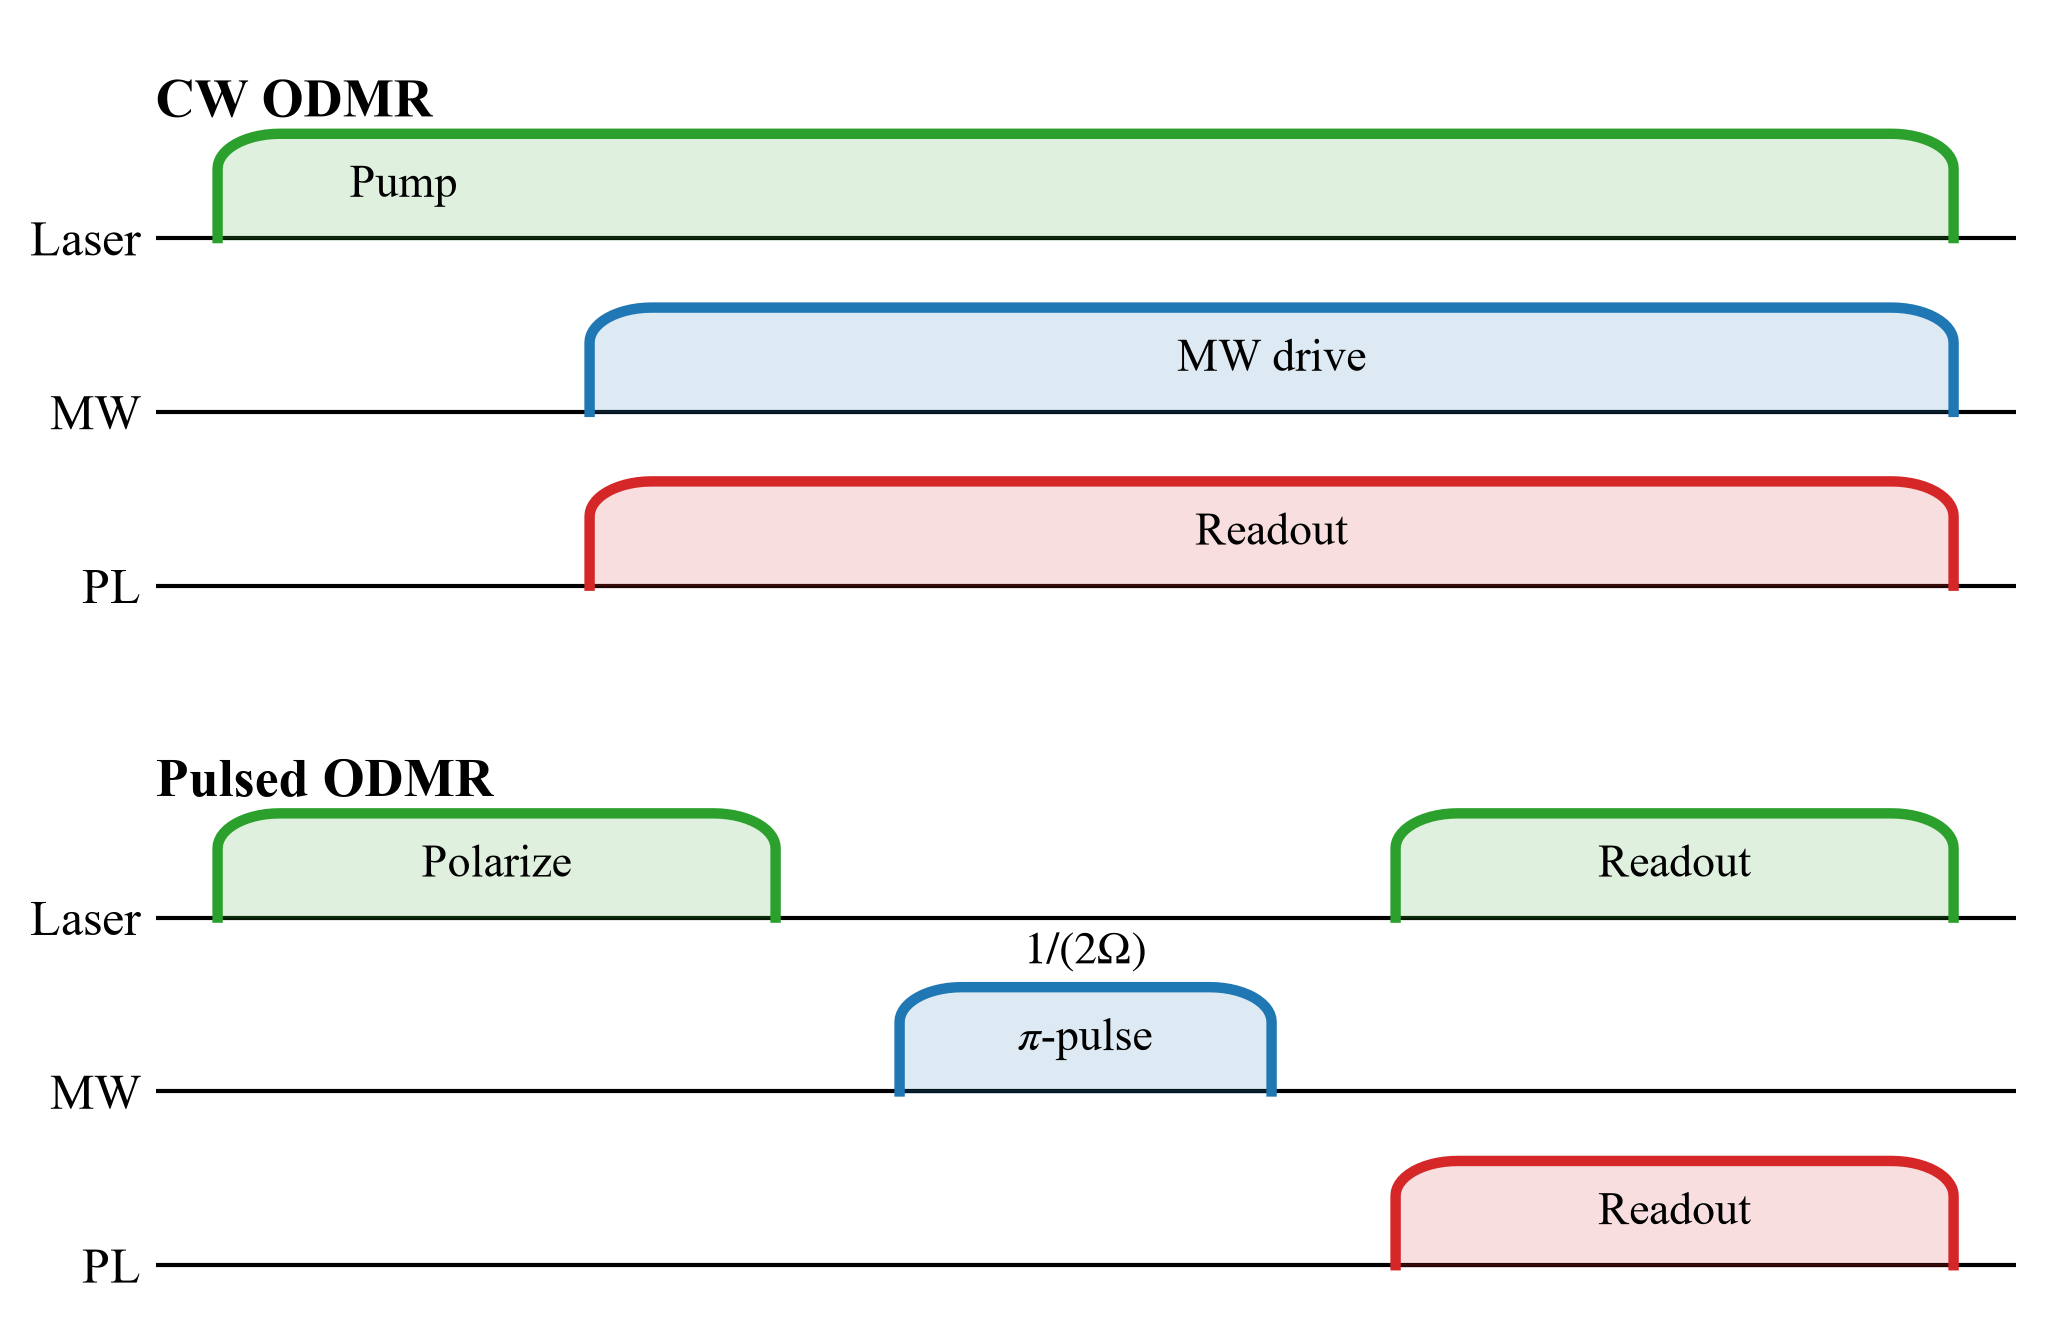
\includegraphics[width=\linewidth]{odmr_sequence}
\caption{Laser and microwave sequences of CW and pulsed ODMR. \tbd{Caption to follow the figure.}}
\label{fig:sequences}
\end{figure}

\paragraph{CW ODMR.} In continuous-wave ODMR the laser and the microwave drive act on the spin continuously and at the
same time, and the PL is read out while the drive is on (Fig.~\ref{fig:sequences}). The laser keeps pumping the spin
back into $m_s=0$ while the drive keeps rotating it away, so every optical reset starts a new Rabi oscillation, and
the PL, collected over many such cycles, reports Eq.~\eqref{eq:rabi} averaged over the time $T$ between resets.
When the drive acts for many Rabi periods between resets, $\Omega_{\rm gen} T\gg1$, the oscillating factor averages to
$\tfrac12$,
\begin{equation}
  \bar P_{-1}(\Delta)=\frac{\Omega^2}{\Omega_{\rm gen}^2}\,\frac1T\int_0^T\sin^2\!\big(\pi\Omega_{\rm gen} t\big)\,dt
  \;\longrightarrow\;\frac12\,\frac{\Omega^2}{\Omega^2+\Delta^2}.
  \label{eq:cw-lorentzian}
\end{equation}
The average only renormalizes the amplitude; the line shape is that of the prefactor, a Lorentzian in the detuning
$\Delta$ of half width $\Omega$. This is the microwave contribution to the width, power broadening: the stronger the
drive, the further off resonance it still flips the spin. With the laser treated as two rates rather than a reset
(Sec.~\ref{sm:cw-pumping}), the line stays a Lorentzian, with the half width of Eq.~\eqref{eq:linewidth} of the
main text.

\paragraph{Pulsed ODMR} is a technique that removes the laser from the width of the line \cite{dreau2011}. In CW ODMR the
laser that reads the spin out also broadens the line through $\Gamma_c$, and narrowing it means lowering both powers
and with them the contrast and the PL. Pulsed ODMR separates the two in time: a laser pulse polarizes the spin into
$m_s=0$, the laser is switched off while a single microwave $\pi$-pulse of duration $t_\pi=1/(2\Omega)$ is applied,
and a second laser pulse reads the spin out (Fig.~\ref{fig:sequences}). The pulse fully inverts the spin on
resonance, and Eq.~\eqref{eq:rabi} at $t=t_\pi$ gives (Sec.~\ref{sm:pulsed})
\begin{equation}
  P_{-1}^{\pi}(\Delta)=\frac{\Omega^2}{\Omega_{\rm gen}^2}\,\sin^2\!\Big(\frac{\pi}{2}\,\frac{\Omega_{\rm gen}}{\Omega}\Big).
  \label{eq:pulsed}
\end{equation}
This line is not a Lorentzian. Its width is the Fourier limit of the pulse, $\sim1/t_\pi$, down to $\sim1/T_2^*$,
where the spread of the transition frequency sets it, and it has side lobes up to 12\% of the depth: dips where there
is no resonance, a hazard for a search.

% Code: NVCenterPulsedDriveModel (spectra/nv_center_drive.py) evaluates Eq. (rabi) at the pulse time with the
% Gaussian T2* average; NVCenterCWDriveModel broadens with MW power only, gamma = gamma_0 sqrt(1 + s_MW),
% gamma_0 = 150 kHz fixed, i.e. no optical term. The SNR x window study uses a fixed linewidth (no drive),
% consistent with one Gamma.

\subsection{Terms left out of the line model}

The Hamiltonian of Eq.~\eqref{eq:hamiltonian} drops the strain term $E(S_x^2-S_y^2)$, since it is a small correction
when $\gamma_e B_z\gg E$.

Each nuclear projection $m_I$ gives its own copy of the line, shifted by
$A_\parallel m_I$ (Eq.~\eqref{eq:transitions}) and weighted by the population of that $m_I$, so the observed
spectrum is a sum of $2I+1$ lines. Two cases reduce it to the single line of Eq.~\eqref{eq:signal}. Near the
excited-state level anticrossing the nitrogen nuclear spin is polarized into a single $m_I$ \cite{jacques2009}: only
one line remains, and its fixed offset $A_\parallel m_I$ is absorbed into $f_-$. When the line is much wider than
the hyperfine spacing, $\Gamma\gg|A_\parallel|$, the lines merge into one.

Equation~\eqref{eq:signal} also leaves out the $f_+$ line. The drive window lies below $D$ and holds $f_-$ only, but
the tail of the $f_+$ line, $2\delta_Z$ higher, adds $C\gamma^2/[\gamma^2+(f-f_+)^2]$ inside it: at $f_-$ a fraction
$\gamma^2/(\gamma^2+4\delta_Z^2)$ of the contrast $C$, i.e.\ 20\% at $\delta_Z=\gamma$ and below 1\% for
$\delta_Z\gtrsim5\gamma$. Equation~\eqref{eq:signal} assumes $\delta_Z\gg\gamma$; small Zeeman shifts, where the two
lines overlap, are outside the scope of this work. The same tail raises the on-resonance depth to
$C[1+\gamma^2/(\gamma^2+4\delta_Z^2)]$, so the SNR $C/\sigma$ of Eq.~\eqref{eq:snr} is the $\delta_Z\gg\gamma$ limit
of the on-resonance SNR.

\subsection{CW line with optical pumping}
\label{sm:cw-pumping}

Eq.~\eqref{eq:cw-lorentzian} treats the laser only as a reset, which is too
crude when the resets are frequent. The laser acts on the spin through two rates, both set by how often the center
goes through an optical cycle: it pumps the spin back toward $m_s=0$, at a rate $\Gamma_p$, and each cycle destroys
the phase between $m_s=0$ and $m_s=-1$, at a rate $\Gamma_c$. The two rates share a cause but are not equal. A cycle
that excites the center destroys the phase whatever happens next, since in the excited state the spin evolves under
a different Hamiltonian and the decay path records its state; only the cycles that pass through the singlet move
population into $m_s=0$. Every pumping cycle therefore destroys the phase, but not every phase-destroying cycle
pumps, and $\Gamma_c$ exceeds $\Gamma_p$.
% The ordering Gamma_c > Gamma_p follows Dreau et al. (2011), whose saturated values differ by about an order of
% magnitude. Verify the values there before quoting numbers.
The spin's environment adds rates of its own, independent of the laser: its longitudinal relaxation $1/T_1$ adds
to $\Gamma_p$ and its homogeneous dephasing $1/T_2$ adds to $\Gamma_c$, giving the total rates
$\Gamma_1=\Gamma_p+1/T_1$ for the populations and $\Gamma_2=\Gamma_c+1/T_2$ for the coherence of
Eq.~\eqref{eq:linewidth}. At the laser powers of CW ODMR both environmental rates are slow against the optical ones,
$\Gamma_1\approx\Gamma_p$ and $\Gamma_2\approx\Gamma_c$, but the derivation below holds for any values of the totals.
The slow spread of the transition frequency, which sets $T_2^*$, is not a rate of this kind and is treated
separately below. The microwave enters only through its angular Rabi
frequency $\Omega_R=2\pi\Omega$. The competition between the two is clearest in terms of populations. A drive whose
coherence is destroyed at the rate $\Gamma_2$ no longer produces Rabi oscillations; it moves population between
$m_s=0$ and $m_s=-1$, in both directions alike, at the rate
\begin{equation}
  W(\Delta)=\frac{\Omega_R^2\,\Gamma_2}{2\big[\Gamma_2^2+(2\pi\Delta)^2\big]}
  =\frac{\Omega_R^2}{2\Gamma_2}\,\frac{\Gamma_2^2}{\Gamma_2^2+(2\pi\Delta)^2},
  \label{eq:transfer-rate}
\end{equation}
a Lorentzian of peak $\Omega_R^2/2\Gamma_2$ and half width $\Gamma_2/2\pi$ in Hz. The laser, helped by $T_1$, returns
population from $m_s=-1$ at the rate $\Gamma_1$, so with $P_0=1-P_{-1}$ the population of $m_s=-1$ obeys
\begin{equation*}
  \dot P_{-1}=W\,(P_0-P_{-1})-\Gamma_1P_{-1}=W-(2W+\Gamma_1)\,P_{-1}.
\end{equation*}
In steady state, inserting Eq.~\eqref{eq:transfer-rate} and then ordering the terms of the denominator,
\begin{equation}
  \begin{aligned}
  P_{-1}^{\rm ss}(\Delta)&=\frac{W}{2W+\Gamma_1}
  =\frac12\,\frac{\Omega_R^2\,\Gamma_2}{\Omega_R^2\,\Gamma_2+\Gamma_1\big[\Gamma_2^2+(2\pi\Delta)^2\big]}\\
  &=\frac12\,\frac{\Omega_R^2\,\Gamma_2/\Gamma_1}{(2\pi\Delta)^2+\Gamma_2^2+\Omega_R^2\,\Gamma_2/\Gamma_1},
  \end{aligned}
  \label{eq:bloch-ss}
\end{equation}
the same as the steady state of the full Bloch equations \cite{dreau2011}. It reduces to
Eq.~\eqref{eq:cw-lorentzian} when the two rates are equal and small against $\Omega_R$. The last form is a
Lorentzian in $2\pi\Delta$ whose squared half width is the constant in its denominator, which gives
Eq.~\eqref{eq:linewidth}.

The first term of Eq.~\eqref{eq:linewidth} is the width without drive, set by the loss of coherence. The
second is power broadening by the microwave: a strong drive saturates the transfer, $W\gg\Gamma_1$, already on the
tails of the line, and the line widens until $W$ there has fallen to about the pumping rate. The depth of the line,
Eq.~\eqref{eq:bloch-ss} at $\Delta=0$, is
\begin{equation*}
  P_{-1}^{\rm ss}(0)=\frac12\,\frac{\Omega_R^2}{\Omega_R^2+\Gamma_1\Gamma_2}:
\end{equation*}
it grows with the microwave power, toward $\tfrac12$, and falls with the laser power, which repolarizes the spin
before the drive can flip it.

\paragraph{Optical saturation.} The two laser rates grow with the laser power, but not without limit. The optical
transition is itself a two-level system: the laser excites the center at a rate proportional to its intensity
$I_{\rm opt}$, and the excited state decays in its lifetime $\tau_e$. In steady state the excited population is
$s/(1+s)$, with the saturation parameter $s=I_{\rm opt}/I_{\rm sat}$ the ratio of the excitation rate to the decay
rate $1/\tau_e$. At low power it grows linearly with $s$; at high power it levels off, because a center cannot be
excited again before it has decayed. The rate of optical cycles is this population divided by $\tau_e$, and both
laser rates follow it, $\Gamma_{p,c}=\Gamma_{p,c}^\infty\,s/(1+s)$ \cite{dreau2011}, with $\Gamma_{p,c}^\infty$ their
values at full saturation. Raising the laser power therefore both widens and flattens the line, up to saturation.
% Dreau et al. (2011) Eq. 11 quotes the same width as Gamma_c^inf/(2 pi) sqrt((s/(1+s))^2 + Omega_R^2/(Gamma_p^inf
% Gamma_c^inf)) and calls it the FWHM; with Gamma_{p,c} = Gamma^inf s/(1+s) this is Eq. (linewidth) up to their
% factor-2 convention for the rates. Check before quoting numbers.

\paragraph{Spin bath in the CW line.} The local fields of the spin bath, mostly the $^{13}$C nuclear spins, shift
the transition by a random offset $\xi$ that changes slowly, over times much longer than the repolarization time
$1/\Gamma_p$. The spin therefore reaches the steady state of Eq.~\eqref{eq:bloch-ss} at the detuning $\Delta-\xi$
before $\xi$ changes, and a measurement that averages over many values of $\xi$ records that steady state convolved
with their distribution, the same average as Eq.~\eqref{eq:pulsed-t2star} below. For a Gaussian distribution of
standard deviation $\sigma_\xi=1/(\sqrt2\,\pi T_2^*)$ the CW line is a Voigt profile: the Lorentzian of
Eq.~\eqref{eq:bloch-ss}, of half width $\gamma$, convolved with a Gaussian of width $\sigma_\xi$. When
$\gamma\gg\sigma_\xi$ it is the Lorentzian of Eq.~\eqref{eq:signal}; when the laser and microwave powers are
lowered until $\gamma\lesssim\sigma_\xi$, the line stops narrowing at a width $\sim1/T_2^*$, as the pulsed line does.
In either case it is one dip with one total width, which is the width inferred in Sec.~\ref{sec:methods} of the main
text; the simulations use a pseudo-Voigt approximation to this profile.

\subsection{Pulsed line}
\label{sm:pulsed}

The $\pi$-pulse length is chosen so that on resonance, where the spin oscillates at
$\Omega$, it is fully inverted: $\pi\Omega t_\pi=\pi/2$. Off resonance it oscillates at $\Omega_{\rm gen}$ instead, so
the argument of the sine in Eq.~\eqref{eq:rabi} at $t=t_\pi$ is $\pi\Omega_{\rm gen} t_\pi=(\pi/2)\,\Omega_{\rm gen}/\Omega$,
which gives Eq.~\eqref{eq:pulsed}. On resonance $\Omega_{\rm gen}=\Omega$ and the inversion is complete. For
$|\Delta|\gg\Omega$, $\Omega_{\rm gen}\approx|\Delta|$ and
$P_{-1}^{\pi}\approx\sin^2(\pi\Delta t_\pi)/(2\Delta t_\pi)^2$, the power spectrum of a rectangular pulse of length
$t_\pi$: far from resonance the spin responds to the frequency content of the pulse. The line vanishes wherever
$\Omega_{\rm gen}=2\Omega,4\Omega,\dots$, i.e.\ at $|\Delta|=\sqrt3\,\Omega,\sqrt{15}\,\Omega,\dots$: there the spin
completes a whole number of full Rabi cycles during the pulse and returns to $m_s=0$. Between the zeros lie side
lobes that decay as $\Omega^2/\Omega_{\rm gen}^2$; the first, near $\Omega_{\rm gen}=3\Omega$ at $|\Delta|\approx2.7\,\Omega$,
is 12\% of the depth.

\paragraph{Inhomogeneous broadening.} The transition frequency of the spin is not sharp: slowly fluctuating local
fields, mostly from the bath of $^{13}$C nuclear spins, shift it by a random offset $\xi$ that is fixed during one
pulse but changes from one repetition of the sequence to the next. A measurement averages many repetitions, each
driven at the detuning $\Delta-\xi$ instead of $\Delta$, so the measured line is Eq.~\eqref{eq:pulsed} averaged over
the distribution of $\xi$, i.e.\ convolved with it. For a Gaussian distribution of standard deviation $\sigma_\xi$,
\begin{equation}
  \bar P_{-1}^{\pi}(\Delta)=\int P_{-1}^{\pi}(\Delta-\xi)\,\frac{e^{-\xi^2/2\sigma_\xi^2}}{\sqrt{2\pi}\,\sigma_\xi}\,d\xi .
  \label{eq:pulsed-t2star}
\end{equation}
The width $\sigma_\xi$ is what $T_2^*$ measures. A free spin precessing at the offset $\xi$ picks up the phase
$2\pi\xi t$, and the average of $e^{2\pi i\xi t}$ over the Gaussian is the coherence envelope
$e^{-2\pi^2\sigma_\xi^2t^2}$. $T_2^*$ is defined by writing this envelope as $e^{-(t/T_2^*)^2}$, so
$\sigma_\xi=1/(\sqrt2\,\pi T_2^*)$. For $t_\pi\ll T_2^*$ the spread is small against $\Omega$ and the line is that of
Eq.~\eqref{eq:pulsed}. For $t_\pi\gtrsim T_2^*$ the Gaussian dominates: the zeros and side lobes are washed out, the
line stops narrowing at a width $\sim1/T_2^*$, and the depth falls because the pulse no longer inverts every
frequency class \cite{dreau2011}.

\paragraph{Readout.} While the microwave pulse is on, the laser is off and the spin relaxes only through $T_1$, which
is much longer than $t_\pi$, and dephases through the spread already included in Eq.~\eqref{eq:pulsed-t2star}. The
readout is different: the laser that reads the spin out also repolarizes it, so the PL difference between $m_s=0$
and $m_s=-1$ lasts only for the repolarization time $\tau_p$. Taking the repolarization as a single exponential, a
spin flipped with probability $P_{-1}$ emits, a time $t$ into the readout pulse, PL at the rate
$\Phi_0\,[1-c\,P_{-1}\,e^{-t/\tau_p}]$, where $\Phi_0$ is the rate of $m_s=0$ and $c$ the fractional PL drop of
$m_s=-1$ at the start of the readout. The recorded PL is this rate integrated over a readout window of length $t_r$,
normalized to the same integral with no flip,
\begin{equation}
  \begin{aligned}
  \mu&=1-\frac{1}{t_r}\int_0^{t_r}c\,P_{-1}\,e^{-t/\tau_p}\,dt\\
  &=1-c\,\frac{\tau_p}{t_r}\big(1-e^{-t_r/\tau_p}\big)\,\bar P_{-1}^{\pi}(\Delta) ,
  \end{aligned}
  \label{eq:pulsed-readout}
\end{equation}
with $P_{-1}=\bar P_{-1}^{\pi}$ of Eq.~\eqref{eq:pulsed-t2star}. The integration leaves the line shape unchanged and
sets only its depth: the contrast is $C=c\,(\tau_p/t_r)(1-e^{-t_r/\tau_p})$. A longer window collects more photons,
$N_{\rm ph}\propto t_r$, but dilutes the contrast, so the single-shot signal-to-noise ratio
$C\sqrt{N_{\rm ph}}\propto(1-e^{-t_r/\tau_p})/\sqrt{t_r/\tau_p}$ is largest at $t_r\approx1.26\,\tau_p$.


% =====================================================================
\section{Bounds for a global search}
\label{sm:prior}
% =====================================================================

This section supports Sec.~\ref{sec:global}: why the van Trees bound does not apply to a uniform window, the
Ziv--Zakai bound that replaces it, the two search bounds, the reach of a measurement and the best probe spacing,
the posterior at detection, and the conditions under which van Trees applies again after detection. Throughout,
$\bar\sigma_\theta^2(n)$ is the mean squared error of Eq.~\eqref{eq:bayes-mse}, averaged over the noise and over
$\theta$ uniform on the window of width $W$.

\paragraph{Why the window breaks van Trees.} For a prior density $p(\theta)$, the van Trees inequality
\cite{vantrees1968,gill1995} bounds the mean squared error of any estimator by
\begin{equation*}
  \bar\sigma_\theta^2(n)\ \ge\ \big(J(p)+nI_{\rm max}\big)^{-1},\qquad
  J(p)=\int\frac{p'(\theta)^2}{p(\theta)}\,d\theta .
\end{equation*}
A uniform window drops from $1/W$ to zero at its edges, so $J(p)$ is infinite and the inequality reduces to
$\bar\sigma_\theta\ge0$: true, but empty. The inverse variance $12/W^2$ cannot simply take its place, since
$J(p)\ge1/\mathrm{Var}(\theta)$ with equality only for a Gaussian. For a signal linear in $\theta$,
$(12/W^2+nI_{\rm max})^{-1/2}$ is the error of the best \emph{linear} estimator, which the best estimator beats.
Table~\ref{tab:sm-prior} gives the size of the effect, computed numerically for a measurement
$y=\theta+\varepsilon$ with $\varepsilon$ Gaussian of variance $1/(nI_{\rm max})$: the best estimator lies up to
$4.4\%$ below the additive curve, around $nI_{\rm max}W^2\approx100$, and the two agree at both ends.

\begin{table}[h]
\centering
\caption{Linear signal, uniform window. Ratio of two curves to the root of the best achievable mean squared error,
$\bar\sigma_{\rm best}$, as a function of the measured information $nI_{\rm max}W^2$. Additive: the van Trees form
with $J_0=12/W^2$, $(12/W^2+nI_{\rm max})^{-1/2}$. ZZ: the Ziv--Zakai bound, Eq.~\eqref{eq:sm-zz-linear}.}
\label{tab:sm-prior}
\begin{tabular}{lccccccc}
\hline
$nI_{\rm max}W^2$ & 1 & 10 & 30 & 100 & 300 & $10^3$ & $10^4$\\
\hline
additive$/\bar\sigma_{\rm best}$ & 0.999 & 1.009 & 1.032 & 1.044 & 1.036 & 1.024 & 1.009\\
ZZ$/\bar\sigma_{\rm best}$ & 0.932 & 0.923 & 0.956 & 0.980 & 0.990 & 0.995 & 0.998\\
\hline
\end{tabular}
\end{table}

\paragraph{The Ziv--Zakai bound.} The Ziv--Zakai bound \cite{zivzakai1969,bell1997} turns estimation into a set of
binary decisions. Take two positions a distance $h$ apart, $\theta$ and $\theta+h$, equally likely a priori, and let
$P_{\min}(\theta,\theta+h)$ be the smallest probability of a wrong decision that any test on the data can reach
between a dip at one and a dip at the other. Two steps give the bound. First, for the error $e=\hat\theta_n-\theta$
of any estimate,
\begin{equation*}
  \bar\sigma_\theta^2(n)=\mathbb E\big[e^2\big]=\frac12\int_0^\infty h\,\Pr\big(|e|\ge h/2\big)\,dh ,
\end{equation*}
which follows from $e^2=\int_0^{2|e|}(h/2)\,dh$, the average running over $\theta$ and the noise as in
Eq.~\eqref{eq:bayes-mse}. Second, the estimate is itself a test: decide for whichever of $\theta$ and $\theta+h$ lies
closer to $\hat\theta_n$. This test errs only if the estimate misses the true position by at least $h/2$, and no test
errs less often than $P_{\min}$, so
\begin{equation*}
  \Pr\big(|e|\ge h/2\big)\ \ge\ G(h)=\int\big[p(\theta)+p(\theta+h)\big]\,P_{\min}(\theta,\theta+h)\,d\theta .
\end{equation*}
Together,
\begin{equation}
  \bar\sigma_\theta^2(n)\ \ge\ \frac12\int_0^\infty h\,G(h)\,dh .
  \label{eq:sm-zz}
\end{equation}
Pairs that the data cannot tell apart thus add to the error in proportion to their distance. The original bound
also replaces $G$ by the smallest nonincreasing function above it, which can only raise the right-hand side; we do
not need it. The bound needs no derivative of $p$, so the edges of the window do not break it. Before any
measurement no test does better than a guess, $P_{\min}=\tfrac12$, and for the uniform prior $G(h)=(W-h)/W$, so
\begin{equation*}
  \bar\sigma_\theta^2(0)\ \ge\ \frac12\int_0^W h\,\frac{W-h}{W}\,dh=\frac{W^2}{12},
\end{equation*}
which is Eq.~\eqref{eq:prior}: the bound starts at the true prior error. For the linear signal,
$P_{\min}=Q\big(h\sqrt{nI_{\rm max}}/2\big)$ with $Q$ the Gaussian tail, which falls with $h$, and
\begin{equation}
  \bar\sigma_\theta^2(n)\ \ge\ \int_0^W h\Big(1-\frac hW\Big)\,Q\Big(\frac{h\sqrt{nI_{\rm max}}}{2}\Big)\,dh ,
  \label{eq:sm-zz-linear}
\end{equation}
which tends to $1/(nI_{\rm max})$ once $nI_{\rm max}W^2\gg1$, the data limit of Eq.~\eqref{eq:vantrees}. It lies within $8\%$ of the best achievable error at every $n$
(Table~\ref{tab:sm-prior}).

\paragraph{Search with a dip of finite reach.} Take the high-SNR idealization of the elimination model: a
measurement at $d$ reports the dip, without error, if and only if the dip lies within the probe cell of width
$\Delta d$ around $d$, and reports the baseline otherwise. Before its first detection every outcome of a run is the
baseline, whatever $\theta$ is, so any strategy, adaptive or not, has measured at a sequence $d_1,\dots,d_n$ fixed
in advance up to that point: each choice depends only on outcomes that are all the same. These $n$ probes cover a set
$C_n$ of measure at most $n\Delta d$; let $U$ be the rest of the window, of measure $L\ge W-n\Delta d$. If both
$\theta$ and $\theta+h$ lie in $U$, the data are the same under the two hypotheses and $P_{\min}=\tfrac12$. Keeping
only these pairs, with $p=1/W$,
\begin{equation*}
  G(h)\ \ge\ \frac2W\cdot\frac12\,\big|U\cap(U-h)\big|=\frac{\big|U\cap(U-h)\big|}{W},
\end{equation*}
where $|U\cap(U-h)|$ is the measure of the positions $\theta$ with both $\theta$ and $\theta+h$ in $U$, and
Eq.~\eqref{eq:sm-zz} gives
\begin{equation*}
  \bar\sigma_\theta^2(n)\ \ge\ \frac{1}{2W}\int_0^\infty h\,\big|U\cap(U-h)\big|\,dh
  =\frac{L^2}{4W}\,\mathbb E\,|X-Y| ,
\end{equation*}
with $X,Y$ independent and uniform on $U$. With $F$ their distribution function,
$\mathbb E|X-Y|=2\int F(1-F)\,dx$, and since $F$ grows by at most $dx/L$ over a step $dx$,
$\int F(1-F)\,dx\ge L\int_0^1u(1-u)\,du=L/6$, with equality only when $U$ is an interval. Hence
\begin{equation*}
  \bar\sigma_\theta^2(n)\ \ge\ \frac{L^3}{12\,W}\ \ge\ \frac{(W-n\Delta d)^3}{12\,W},
\end{equation*}
Eq.~\eqref{eq:search-mean}. The elimination model, which probes contiguously from one edge, meets
it: no strategy searches a window faster in this limit. A strategy that probes in a scattered order leaves $U$ in
pieces, and its mean error at the same $n$ is larger.

\paragraph{Search at any SNR.} At lower SNR a single measurement no longer decides, and the argument above no longer
applies, since an adaptive strategy now branches on noisy outcomes. A change-of-measure argument
\cite{garivier2019} bounds it instead. It rests on the same idea as the Ziv--Zakai bound, a binary test, but the
alternative to a dip at $\theta$ is now no dip at all, and the evidence for telling them apart is counted by the
Kullback--Leibler divergence. Let $P_\theta$ be the law of all the data of a run with the dip at $\theta$,
and $P_0$ the law with no dip at all, the strategy being the same. In each measurement the outcome is Gaussian with
variance $\sigma^2/k$ and mean shifted by the dip depth at the drive frequency,
$s(d;\theta)=C\gamma^2/[\gamma^2+(d-\theta)^2]$. Each drive frequency $d_i$ is chosen from the past outcomes by the
same rule under both laws, so the chain rule of the Kullback--Leibler divergence gives, for adaptive strategies too,
\begin{equation*}
  D_{\rm KL}(P_0\,\|\,P_\theta)=\mathbb E_0\Big[\sum_{i=1}^{n}\frac{k\,s(d_i;\theta)^2}{2\sigma^2}\Big].
\end{equation*}
Each term is the divergence of one measurement, for two Gaussians of equal variance the squared shift of the mean
over twice the variance. The expectation is under $P_0$, where the choices cannot depend on $\theta$. Averaged over
$\theta$ uniform on the window, at any $d$ one measurement adds at most
\begin{equation*}
  \begin{aligned}
  \bar\kappa&=\frac1W\int\frac{k\,s(d;\theta)^2}{2\sigma^2}\,d\theta
  \ \le\ \frac{k\,C^2\gamma^4}{2\sigma^2W}\int_{-\infty}^{\infty}\frac{dv}{(\gamma^2+v^2)^2}\\
  &=\frac{k\,C^2\gamma^4}{2\sigma^2W}\,\frac{\pi}{2\gamma^3}=\frac{\pi\gamma\,k\,\mathrm{SNR}^2}{4W},
  \end{aligned}
\end{equation*}
with $v=d-\theta$, the integral over the whole line bounding the one over the window. Hence
\begin{equation*}
  \frac1W\int D_{\rm KL}(P_0\,\|\,P_\theta)\,d\theta\ \le\ n\bar\kappa .
\end{equation*}
Now let $A_\theta$ be the event $|\hat\theta_n-\theta|\le t$, with probabilities $p_0(\theta)=P_0(A_\theta)$ and
$p_\theta=P_\theta(A_\theta)$. Under $P_0$ the estimate does not depend on $\theta$, so the average of $p_0(\theta)$
over the window is at most $2t/W$. By data processing and the joint convexity of the binary divergence
$\mathrm{kl}(p,q)=p\ln\frac pq+(1-p)\ln\frac{1-p}{1-q}$, the averages $\bar p_0$ and $\bar p$ satisfy
$\mathrm{kl}(\bar p_0,\bar p)\le n\bar\kappa$. With $\mathrm{kl}(p,q)\ge(1-p)\ln\frac{1}{1-q}-\ln2$, the fraction
of runs whose estimate is still more than $t$ from the dip is
\begin{equation*}
  1-\bar p\ \ge\ \exp\!\Big(-\frac{n\bar\kappa+\ln2}{1-2t/W}\Big),
  \qquad \bar\sigma_\theta^2(n)\ \ge\ t^2\,(1-\bar p).
\end{equation*}
This holds for every $0<t<W/2$. With $a=1+\ln2+n\bar\kappa$, the choice $t=W/2a$ gives
$1/(1-2t/W)=a/(a-1)$, so the exponent is $-a$ and
\begin{equation*}
  \bar\sigma_\theta^2(n)\ \ge\ \frac{W^2}{4a^2}\,e^{-a}=\frac{W^2}{8e}\,\frac{e^{-n\bar\kappa}}{(1+\ln2+n\bar\kappa)^2},
\end{equation*}
which is Eq.~\eqref{eq:search-bound}. It keeps the rate $e^{-n\bar\kappa}$ and holds at every $n$. Computed
numerically, it lies within a factor $1.03$ of the bound maximized over $t$ for $n\bar\kappa\le1$, and within $1.42$
for $n\bar\kappa\le50$. The fixed choice $t=W/4$ gives the simpler $W^2e^{-2n\bar\kappa}/64$, but at half the rate.
The search therefore takes at least of order $1/\bar\kappa$ measurements, Eq.~\eqref{eq:search-cost}. The bound has
no factor $\ln(W/\Gamma)$, and none is needed. A strategy that averages a fixed number of shots at every probe
position must raise its detection threshold with the number of positions to keep false alarms rare, and pays about
$\ln(W/\Delta d)$ more, Eq.~\eqref{eq:sm-fixed-cost} below. A sequential test spends its shots where they are
needed: it drops a position as soon as it looks like the baseline and measures again only where the outcome is
ambiguous, so it needs strong evidence only to confirm a dip, and avoids most of the factor \cite{malloy2014}. A
Bayesian strategy goes further: its posterior combines the outcomes at neighboring positions, which the tails of the
dip reach as well, and lowers the weight of a position with each outcome that looks like the baseline instead of
excluding it at once. At high SNR $1/\bar\kappa$ falls below $W/\Delta d$, one measurement per probe position, and the
finite-reach bound above is the one that binds.

\paragraph{The reach of a measurement.} The finite-reach bound treats the dip as invisible beyond its probe cell.
The probe spacing $\Delta d$ must make that true: a dip anywhere in a cell, even at its edge, a distance
$\Delta d/2$ from the probe, must be detected, while none of the $M=W/\Delta d$ cells on the baseline may be taken
for a dip. A probe declares a dip when its drop exceeds a threshold of $z_\alpha$ noise standard deviations
$\sigma/\sqrt k$. For Gaussian noise the largest of $M$ baseline draws is about $\sqrt{2\ln M}$, so keeping false
alarms rare needs $z_\alpha\approx\sqrt{2\ln M}$. A dip at the cell edge is
$C\gamma^2/[\gamma^2+(\Delta d/2)^2]=C/[1+(\Delta d/\Gamma)^2]$ deep, and is missed with a small probability only if
its drop exceeds the threshold by a further $z_\beta$. With $z=z_\alpha+z_\beta$,
\begin{equation}
  \frac{\sqrt k\,\mathrm{SNR}}{1+(\Delta d/\Gamma)^2}\ \ge\ z
  \quad\Longrightarrow\quad
  \Delta d=\Gamma\sqrt{\frac{\sqrt k\,\mathrm{SNR}}{z}-1}.
  \label{eq:sm-reach}
\end{equation}
A single measurement detects anything only for $\sqrt k\,\mathrm{SNR}>z$. The reach is below the line width for
$\sqrt k\,\mathrm{SNR}<2z$, where only the core of the dip stands out, and above it at higher SNR, where the
Lorentzian tails do too and a measurement rules out more than a line width. The change-of-measure bound uses the
Lorentzian itself and does not depend on this choice.

\paragraph{The best spacing.} At lower SNR a probe repeats $m$ measurements at the same drive frequency, which
multiplies $k$ by $m$ in Eq.~\eqref{eq:sm-reach}. More repeats widen the reach and so need fewer probes; the search
costs $m\,W/\Delta d$ measurements. With $a=\sqrt k\,\mathrm{SNR}/z$ and $u=\sqrt m\,a$, the cost per unit of window
is
\begin{equation*}
  \frac{m}{\Delta d}=\frac{1}{\Gamma\,a^2}\,\frac{u^2}{\sqrt{u-1}},
\end{equation*}
smallest at $u=4/3$, with $m$ treated as continuous. The best probe then averages just enough for the drop at
$\sqrt m\,\sqrt k\,\mathrm{SNR}=\tfrac43z$, and the best spacing is
\begin{equation*}
  \Delta d_{\rm opt}=\frac{\Gamma}{\sqrt3}\approx0.58\,\Gamma,
\end{equation*}
below the line width: it pays to see only the core of the dip and to take more probes. A spacing wider than
$\Gamma/\sqrt3$ is the best choice only when a single measurement already has $a>4/3$, so that $m=1$ and
$\Delta d$ follows from Eq.~\eqref{eq:sm-reach}. At the optimum the search costs
\begin{equation}
  n_{\rm fixed}=\frac{16\sqrt3}{9}\,\frac{W}{\Gamma}\,\frac{z^2}{k\,\mathrm{SNR}^2}
  \approx1.2\,z^2\,\frac{1}{\bar\kappa},
  \label{eq:sm-fixed-cost}
\end{equation}
with $1/\bar\kappa$ the change-of-measure bound, Eq.~\eqref{eq:search-cost}. With $z^2\approx2\ln M$ this is about
$2.4\ln(W/\Delta d)$ times the bound: the factor that a sequential test avoids.

\paragraph{The detection posterior.} Let the detecting measurement be at the center $d$ of its cell, with the dip
uniform over the cell; we neglect the weak information that the non-detection at the previous probe carries about the
near edge of the cell. The outcome $y$ of the measurement, and with it any detection rule applied to $y$, depends on
$\theta$ only through $|\theta-d|$. The posterior is then symmetric about $d$ and $\mathbb E[\theta\mid y]=d$ for
every $y$, so by the law of total variance
\begin{equation*}
  \mathbb E\big[\mathrm{Var}(\theta\mid y)\big]=\mathrm{Var}(\theta)-\mathrm{Var}\big(\mathbb E[\theta\mid y]\big)
  =\frac{\Delta d^2}{12}-0 ,
\end{equation*}
exactly, at any SNR. The depth of the drop changes only the shape of the posterior. At high SNR it fixes
$|\theta-d|$ to within about $I(\theta)^{-1/2}$, with $I(\theta)$ the Fisher information of Eq.~\eqref{eq:fisher}
of the detecting measurement, and the posterior is two narrow peaks at $d\pm|\theta-d|$.

\paragraph{Restarting van Trees after detection.} Let $\tau$ be the step at which a run declares the dip found,
decided from the run's own data and never from the true $\theta$. Given the data up to $\tau$, the posterior is the
prior of the remaining measurements, and van Trees applied to them, then averaged over runs, gives
$\bar\sigma_\theta^2(n)\ge\mathbb E[(J_\tau+(n-\tau)I_{\rm max})^{-1}]$ with $J_\tau$ the Fisher information of that
posterior. $J_\tau$ is finite: every likelihood is Gaussian in $y$ and so smooth in $\theta$, and the posterior has
none of the hard edges of the idealized cell. Right after detection the two mirror peaks make $J_\tau$ of order $I(\theta)$, far above
$12/\Delta d^2$, while the error is $\Delta d/\sqrt{12}$: the restarted bound is valid but loose until the side is
known. The elimination model therefore restarts with the value that matches the error, $J_\tau=12/\Delta d^2$, a
model value rather than a bound. The measurement that resolves the side is placed at the steepest slope of one of
the two peaks: if that is the true one it adds $I_{\rm max}$, as the model assumes; if not, it sees little of the dip
and adds less, but still tells the side. Once the side is known the posterior is a single peak of variance about
$(I(\theta)+I_{\rm max})^{-1}$, and the restarted bound is tight; the model, which keeps $12/\Delta d^2$ and
discards $I(\theta)$, is conservative from then on, by an amount that ranges from nothing for a dip right under the
probe, where $I(\theta)\approx0$, to $I_{\rm max}$ for one on its flank. The window edges still cut the posterior
off, but where it holds a negligible fraction of its mass, so smoothing them changes the bound by a negligible
amount. The bound is on the error expected given the run's history; the posterior variance of a single run may
fluctuate slightly below it.


% =====================================================================
\section{Expected information gain in search and localize}
\label{sm:eig}
% =====================================================================

Sec.~\ref{sec:eig} of the main text asks two questions of the variance form of the expected information gain,
Eq.~\eqref{eq:eig-var}: (A) when it agrees with the exact gain, and (B) when maximizing it greedily puts the
measurements where the van Trees bound needs them. In refine the answer to both is yes. This section gives the
argument for the two earlier regimes, where both fail.

\paragraph{Search: a two-valued signal.} Before the dip is found the posterior of $\theta$ is spread over the window,
and the predicted signal at $x$ is two-valued: with probability $p$, the posterior mass that would put the dip at $x$,
it is about $1-C$, otherwise 1. Then $\sigma^2_{\rm pred}=p(1-p)C^2$, while the true mutual information is at most the
binary entropy $H_b(p)\le\ln2$. For (A), the variance form keeps growing with SNR where the true gain saturates, so it
overvalues search candidates relative to refine candidates; both peak at $p=\tfrac12$, so they rank search
candidates alike. For (B), the chain-rule argument of Eq.~\eqref{eq:eig-sum} fails, since where one measures changes
what later measurements can gain. Here greedy EIG is only myopically optimal, which is where the strategies of
Sec.~\ref{sec:locators} of the main text differ.

\paragraph{Localize: the variance form chases the tail.} The same two-valued picture holds in the localize stage,
with a different ranking. Once a peak has formed at the dip, a small residual mass $p$ far from it gives a predictive
variance $p(1-p)C^2$ at its location, large at high SNR even for small $p$, while the information it holds is at most
$H_b(p)$, small for small $p$. The variance form therefore keeps spending measurements to remove such distant mass.
This reduces the posterior variance, which the tail dominates (Sec.~\ref{sm:gaussian}) and which is the quantity
Eq.~\eqref{eq:vantrees} constrains, rather than the posterior entropy: in the localize stage the variance rule acts
as a design for the MSE, while a rule built on the information gain would refine the peak sooner and accept the
tail. Whether this explains why localizing costs SBED far more measurements than the bound is a hypothesis we have
not tested.


% =====================================================================
\section{Approach of the posterior to a Gaussian}
\label{sm:gaussian}
% =====================================================================

Eq.~\eqref{eq:eig-fisher} and the reading of $\sigma_\theta$ as a 68\% interval assume a Gaussian posterior. This
section states when that holds for the line of Eq.~\eqref{eq:signal}. There are two separate questions: whether
the posterior has a single peak, and whether that peak is Gaussian. We take the nuisances as known; they add
dimensions but do not change the scaling.

\paragraph{Shape of a single peak.} Let $\ell(\theta)=\ln p(\theta)+\sum_i\ln\mathcal L_i(\theta)$ be the log
posterior and $\hat\theta$ its maximum. Inside the window the uniform prior is flat and only the likelihood
contributes. Expanding about the maximum (Laplace's method \cite{vandervaart1998}),
\begin{equation}
  \ell(\theta)=\ell(\hat\theta)-\frac{J}{2}(\theta-\hat\theta)^2+\frac{\ell'''}{6}(\theta-\hat\theta)^3
  +\frac{\ell''''}{24}(\theta-\hat\theta)^4+\dots,
  \label{eq:laplace}
\end{equation}
with $J=-\ell''(\hat\theta)$, whose expectation is the Fisher information $J_n$ of Sec.~\ref{sec:fisher}. Keeping only
the quadratic term gives a Gaussian of variance $\sigma_\theta^2=1/J$. Over the posterior,
$|\theta-\hat\theta|\sim\sigma_\theta$, so the higher terms change the log density by relative amounts of order
$\ell'''\sigma_\theta^3$ and $\ell''''\sigma_\theta^4$; the first sets the asymmetry of the peak, the second the weight
of its tails.

For Gaussian noise, $\ln\mathcal L(\theta)=-k\,[y-\mu(x;\theta)]^2/2\sigma^2$ up to a constant. Averaged over the
noise, the derivatives are
\begin{equation*}
  \mathbb E[\ell'']=-\sum_i\frac{k\,\mu_i'^2}{\sigma^2}=-J_n,\qquad
  \mathbb E[\ell''']=-3\sum_i\frac{k\,\mu_i'\mu_i''}{\sigma^2},
\end{equation*}
where primes are derivatives with respect to $\theta$ at $x_i$. The line changes on the scale
of its half width $\gamma$, so each further derivative brings a factor of order $1/\gamma$: $\mu''\sim\mu'/\gamma$,
hence $|\ell'''|\lesssim J_n/\gamma$ and $|\ell''''|\lesssim J_n/\gamma^2$. The corrections in Eq.~\eqref{eq:laplace} are
then of relative order
\begin{equation}
  \ell'''\sigma_\theta^3\sim\frac{\sigma_\theta}{\gamma},\qquad \ell''''\sigma_\theta^4\sim\frac{\sigma_\theta^2}{\gamma^2}.
  \label{eq:gauss-corrections}
\end{equation}
A single peak is Gaussian once it is narrow compared with the line, $\sigma_\theta\ll\gamma$. This is an upper
estimate: at the steepest-slope points $\mu''=0$ (there $|\mu'|$ is at its maximum), so for measurements placed there
the cubic term vanishes on average and the corrections start at order $\sigma_\theta^2/\gamma^2$.

In the data limit, $J_n\approx nI_{\rm max}$ with $I_{\rm max}$ of Eq.~\eqref{eq:istar}, and with $\Gamma=2\gamma$,
\begin{equation*}
  \frac{\sigma_\theta}{\gamma}\approx\frac{8}{3\sqrt3}\,\frac{1}{\mathrm{SNR}\sqrt{nk}}
  \approx\frac{1.5}{\mathrm{SNR}\sqrt{nk}} ,
\end{equation*}
so at an SNR of order 10 a few shots on the sides of the dip already make the peak Gaussian.

\paragraph{Linearization of the signal.} The same ratio controls the step from a Gaussian posterior to a Gaussian
prediction used in Eq.~\eqref{eq:eig-fisher}. Expanding the signal over the posterior,
$\mu(x;\theta)=\mu(x;\hat\theta)+\mu'(x)(\theta-\hat\theta)+\tfrac12\mu''(x)(\theta-\hat\theta)^2+\dots$, the
quadratic term relative to the linear one is $\mu''\sigma_\theta/2\mu'\sim\sigma_\theta/\gamma$. Eq.~\eqref{eq:eig-fisher}
therefore holds up to relative corrections of order $\sigma_\theta/\gamma$, and of order $\sigma_\theta^2/\gamma^2$
at the steepest slope.

\paragraph{Leftover mass.} The expansion describes one peak. Early in the localize stage the posterior is instead a mixture: a
peak of weight $1-p$ and width $\sigma_\theta$ at the dip, and a remainder of weight $p$ spread over the part of
the window not yet excluded, of width up to $W$. The variance of the mixture is
\begin{equation*}
  \mathrm{Var}(\theta)\approx(1-p)\,\sigma_\theta^2+p\,s_{\rm r}^2,
\end{equation*}
where $s_{\rm r}^2\lesssim W^2/12$ is the mean squared distance of the remainder from the peak. The remainder
dominates once $p\gtrsim\sigma_\theta^2/s_{\rm r}^2$, i.e.\ roughly $p\gtrsim12(\sigma_\theta/W)^2$, a very small
weight: for $W=20\,\Gamma$ and $\sigma_\theta=0.1\,\Gamma$ it is $3\times10^{-4}$. Until the remainder has fallen below
this, the posterior standard deviation reports the remainder, not the error of the peak, and the posterior is
far from Gaussian: a narrow peak with wide tails. Its entropy, by contrast, is changed by the remainder only by
about $H_b(p)+p\ln(s_{\rm r}/\sigma_\theta)$, which is small for small $p$. This is the difference between the
variance and the information gain discussed in Sec.~\ref{sec:eig}.

The remainder is removed only by measuring where it would place the dip. A measurement within about $\gamma$ of such
a location, when the dip is not there, lowers the log weight of that part of the remainder on average by the
Kullback--Leibler divergence between the two predicted outcomes, $kC^2/2\sigma^2=k\,\mathrm{SNR}^2/2$. Lowering a
weight $p$ to below $12(\sigma_\theta/W)^2$ takes, at each location, about
$2\ln[pW^2/12\sigma_\theta^2]/(k\,\mathrm{SNR}^2)$ measurements, and at least one; a remainder spread over the
whole window has of order $W/\Gamma$ such locations. At high SNR the posterior therefore becomes Gaussian after
about one pass over the remaining window, a cost that grows with $W/\Gamma$ like that of the search.
\tbd{Compare with when the SBED posterior becomes Gaussian in the runs (Results).}


% =====================================================================
\section{Measurements to a target, bandwidth and sensitivity over a run}
\label{sm:speedup}
% =====================================================================

This section derives the number of measurements a sweep and an adaptive strategy need to reach a target
precision, from which the speedup of Eq.~\eqref{eq:speedup} and the bandwidth of Sec.~\ref{sec:sensitivity} of
the main text follow, and the course of the sensitivity over a run.

\paragraph{Sweep.} Where a sweep measures does not depend on what it has learned, so its expected information grows
at the constant rate $I_{\rm sweep}$ of Eq.~\eqref{eq:sweep-info} from its first measurement, and the van Trees bound
for the sweep is $\sigma\approx(\sigma_0^{-2}+nI_{\rm sweep})^{-1/2}$. This has the same $n^{-1/2}$ form as the refine
regime of an adaptive strategy; the two differ in the rate, $I_{\rm sweep}$ against $I_{\rm max}$. A single sweep
reaches this bound only once its posterior has one peak. Until the scan has passed over the dip it learns only that
the dip is not where it has looked, so its error, like that of an adaptive run, stays near $\sigma_0$ and then drops
when the dip is resolved, after about one pass of the window, or several at low SNR. What the sweep lacks is the
phase after that: an adaptive strategy moves its measurements onto the slope, so its rate rises from about
$I_{\rm sweep}$ to $I_{\rm max}$, while the sweep keeps spending a fraction of order $\Gamma/W$ of its measurements on
the line and stays at $I_{\rm sweep}$. Averaged over many passes the steps of the individual runs are smoothed out,
and the error follows the bound with no plateau and no cliff, as observed by \citet{dushenko2020sbed}.

\paragraph{Measurements to a target.} This too is a model of the error, so the window enters through its inverse
variance. An adaptive strategy pays the search cost $n_d$ of the elimination model first and then gains
$I_{\rm max}$ per measurement. Let $\sigma_{\rm tgt}$ (Hz) be the target precision, the standard deviation of $f_-$ at
which a run is considered done. The number of measurements to reach it is
\begin{equation}
  \begin{aligned}
  N_{\rm sweep}(\sigma_{\rm tgt})&=\frac{\sigma_{\rm tgt}^{-2}-\sigma_0^{-2}}{I_{\rm sweep}},\\
  N_{\rm ad}(\sigma_{\rm tgt})&=n_d+\frac{\sigma_{\rm tgt}^{-2}-12/\Delta d^2}{I_{\rm max}},
  \end{aligned}
  \label{eq:n-to-target}
\end{equation}
where the adaptive count follows the elimination model, Eqs.~\eqref{eq:elimination}--\eqref{eq:after-detection}:
$n_d$ measurements to detect the dip, after which the information starts at $12/\Delta d^2$ and grows by
$I_{\rm max}$ per measurement until it reaches $\sigma_{\rm tgt}^{-2}$. The sweep count uses the averaged rate, so it
holds for targets that take more than one pass of the window. The speedup is
$R(\sigma_{\rm tgt})=N_{\rm sweep}/N_{\rm ad}$. For a precise target the refine terms dominate and $R$ tends to
$R_\infty=I_{\rm max}/I_{\rm sweep}$ of Eq.~\eqref{eq:speedup}. For a loose target the search cost $n_d$ dominates
$N_{\rm ad}$ and $R(\sigma_{\rm tgt})<R_\infty$, so the full dependence on window, linewidth, SNR (through $n_d$ at
low SNR) and target is given by Eq.~\eqref{eq:n-to-target}.

\paragraph{Bandwidth.} The time to reach the target is $t_m$ times $N_{\rm ad}(\sigma_{\rm tgt})$, $n_d$ measurements
to find the dip and the rest to refine it:
\begin{equation}
  T(\sigma_{\rm tgt})=t_m\Big[n_d+\frac{\sigma_{\rm tgt}^{-2}-12/\Delta d^2}{I_{\rm max}}\Big].
  \label{eq:bandwidth}
\end{equation}
For a tight target the refine term dominates, $T\approx t_m\sigma_{\rm tgt}^{-2}/I_{\rm max}$, which is the sensitivity
$\eta$ of Eq.~\eqref{eq:sensitivity} again. For a loose target the search term dominates, $T\approx n_d t_m$: the
bandwidth cannot exceed about $1/(n_d t_m)$, whatever the SNR, which is $2\Delta d/(W t_m)$ for a resonance halfway
through the window.

\paragraph{Sensitivity as a function of time.} Eq.~\eqref{eq:sensitivity} is a limit. Read off a run of length $T$,
the product $\eta(T)=\sigma_B(T)\sqrt T$ also carries the search, and its expected course follows from the error
curve of Sec.~\ref{sec:budget} with $n=T/t_m$. During the search the error barely falls, Eq.~\eqref{eq:elimination},
so the product grows,
\begin{equation*}
  \eta(T)=\frac{1}{\gamma_e}\,\frac{W-(T/t_m)\Delta d}{\sqrt{12}}\,\sqrt T\;\propto\;\sqrt T,\qquad T<n_d t_m .
\end{equation*}
Detection drops it by the localize factor, and afterwards, by Eq.~\eqref{eq:after-detection},
\begin{equation}
  \frac{\eta(T)}{\eta}=\Big(1-\frac{n_e\,t_m}{T}\Big)^{-1/2}\approx1+\frac{n_e\,t_m}{2T},
  \qquad T\ge n_d t_m ,
  \label{eq:sensitivity-time}
\end{equation}
with $\eta$ the sensitivity of Eq.~\eqref{eq:sensitivity} and $n_e=n_d-12/(\Delta d^2 I_{\rm max})$. The measurements spent on the search, less the information
that detection supplies, are a fixed debt $n_e$; refine pays it off, so $\eta(T)$ approaches $\eta$ from above and the
excess falls as $1/T$ (Fig.~\ref{fig:sensitivity-time}). A run therefore reports a sensitivity within a fraction
$\epsilon$ of $\eta$ only once $T\gtrsim n_e t_m/2\epsilon$, i.e.\ after about $50\,n_e$ measurements for 1\%. For any
strategy described by $(n_0,q)$, Eq.~\eqref{eq:strategy-numbers} gives the same form,
$\eta(T)\approx(\eta/\sqrt q)\,(1-n_0t_m/T)^{-1/2}$: $q$ sets the floor and $n_0$ how slowly it is reached. The
unbiased Cram\'er--Rao bound $(nI_{\rm max})^{-1/2}$ is the constant $\eta$ at all $T$; the van Trees bound, which
includes the prior, lies below it and rises to it as $\sqrt T$ while $T\lesssim n_c t_m$, but no strategy can follow it
there, since $J_0$ belongs to the window and not to any measurement.

\begin{figure}[t]
\centering
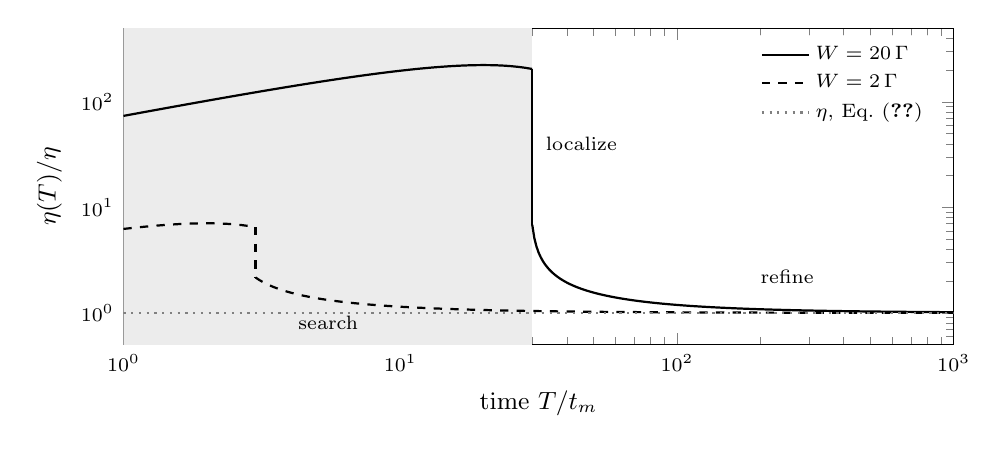
\begin{tikzpicture}
\begin{loglogaxis}[
  width=\linewidth, height=5.6cm,
  xlabel={time $T/t_m$}, ylabel={$\eta(T)/\eta$},
  xmin=1, xmax=1000, ymin=0.5, ymax=500,
  legend style={font=\scriptsize, at={(0.98,0.98)}, anchor=north east, draw=none, fill=white, fill opacity=0.8,
    text opacity=1},
  legend cell align=left,
  label style={font=\small}, tick label style={font=\scriptsize},
]
% Same illustrative values as Fig. budget: SNR = 10, k = 1, Delta x = Gamma/3 -> I* = 168.75 / Gamma^2;
% eta(T)/eta = sigma(n) sqrt(n I*), n = T/t_m.
\fill[gray!15] (axis cs:1,0.5) rectangle (axis cs:30,500);
\node[font=\scriptsize] at (axis cs:5.5,0.8) {search};
\node[font=\scriptsize, anchor=west] at (axis cs:31,40) {localize};
\node[font=\scriptsize] at (axis cs:250,2.2) {refine};
\addplot[thick, domain=1:30, samples=60] {(20 - x/3)/sqrt(12)*sqrt(168.75*x)};
\addlegendentry{$W=20\,\Gamma$}
\addplot[thick, forget plot] coordinates {(30, 205.4) (30, 6.847)};
\addplot[thick, forget plot, domain=30:1000, samples=200] {sqrt(168.75*x/(108 + 168.75*(x-30)))};
\addplot[thick, dashed, domain=1:3, samples=20] {(2 - x/3)/sqrt(12)*sqrt(168.75*x)};
\addlegendentry{$W=2\,\Gamma$}
\addplot[thick, dashed, forget plot] coordinates {(3, 6.495) (3, 2.165)};
\addplot[thick, dashed, forget plot, domain=3:1000, samples=200] {sqrt(168.75*x/(108 + 168.75*(x-3)))};
\addplot[gray, dotted, thick, domain=1:1000, samples=2] {1};
\addlegendentry{$\eta$, Eq.~\eqref{eq:sensitivity}}
\end{loglogaxis}
\end{tikzpicture}
\caption{Expected sensitivity $\eta(T)=\sigma_B(T)\sqrt T$ of an adaptive strategy as a function of the run time,
from the elimination model with the values of Fig.~\ref{fig:budget}. Solid: wide window, $W=20\,\Gamma$; dashed:
narrow window, $W=2\,\Gamma$; dotted: the refine limit $\eta$ of Eq.~\eqref{eq:sensitivity}, which is also the
unbiased Cram\'er--Rao bound. During the search (shaded) $\eta(T)$ grows as $\sqrt T$; detection drops it, and in
refine it approaches $\eta$ from above with an excess $n_e t_m/2T$, Eq.~\eqref{eq:sensitivity-time}. Simulated and
measured runs are shown against $\eta$ in Sec.~\ref{sec:results}.}
\label{fig:sensitivity-time}
\end{figure}


% =====================================================================
\section{Algorithm settings}
\label{sm:algorithm}
% =====================================================================
% Every number below is the code default (nvision/belief/smc_marginal.py, nvision/sim/defaults.py,
% nvision/sim/locs/bayesian/sbed_locator.py, nvision/belief/focus_window.py, nvision/belief/dip_detection.py,
% nvision/sim/locs/search_grid.py).

\paragraph{Particle filter.} The cloud has $N_p=1000$ particles. Every dimension is scaled to $[0,1]$ by its prior
bounds, so one resampling kernel serves all of them; reported values are mapped back to Hz. The cloud is resampled
when the effective sample size $(\sum_i w_i^2)^{-1}$ falls below $0.2\,N_p$, systematically, and then rejuvenated with
the Liu--West kernel,
\begin{equation}
  \psi_i'\sim\mathcal N\big(a\psi_i+(1-a)\bar\psi,\ (1-a^2)\Sigma\big),\qquad a=0.98,
  \label{eq:liuwest}
\end{equation}
with $\psi_i=(\theta_i,\phi_i)$ the whole particle and $\bar\psi$, $\Sigma$ the weighted mean and covariance before
resampling. The diagonal of $\Sigma$ is floored at $(0.01\,e^{-n/25})^2$ of each unit range after $n$ measurements,
and a particle that leaves the unit cube is reflected back into it.

\paragraph{Noise model.} Each particle carries an inverse-gamma posterior on $\sigma^2$ with shape $\alpha$, the same
for every particle because its update does not depend on the residuals, and scale $\beta_i$. The prior is
$\alpha_0=10$, $\beta_0=\alpha_0\sigma_{\rm nom}^2$, with $\sigma_{\rm nom}$ the geometric mean of the prior range of
$\sigma$. Before each measurement both are discounted by $d=0.99$; a measurement $y_n$, the mean of $k$ shots at
$d_n$, then adds $\tfrac12$ to $\alpha$ and $\tfrac12 k\,r_{n,i}^2$ to $\beta_i$, with residual
$r_{n,i}=y_n-\mu(d_n;\theta_i,\phi_i)$, so that after $n$ measurements
$\beta_i=d^n\beta_0+\tfrac12\sum_{t<n}d^{\,n-1-t}k\,r_{t,i}^2$. Old residuals are thus forgotten with a memory of
about $1/(1-d)=100$ measurements, and $\alpha$ saturates at $0.5/(1-d)=50$, about 100 degrees of freedom. With
$\sigma^2$ integrated out, the measurement reweights the particles by the Student-$t$ predictive
\begin{equation}
  w_i\ \propto\ w_i\;t_{2\alpha}\!\Big(y_n;\,\mu(d_n;\theta_i,\phi_i),\,\frac{\beta_i}{k\alpha}\Big),
  \label{eq:smc-update}
\end{equation}
taken with $\alpha$, $\beta_i$ before the update. After a rejuvenation each $\beta_i$ is recomputed from the full
history at the particle's new position.

\paragraph{Initial cloud.} The simulated runs are global searches (Sec.~\ref{sec:prior}): the prior on the Zeeman
shift $\delta_Z$ is uniform over the range the truth is drawn from. \tbd{Tracking runs, with a Gaussian prior and the
truth drawn from that same Gaussian, are not simulated yet.}

\paragraph{Stop rule and budget.} The ceilings on the claimed uncertainty are $100$~kHz for $\theta$, $500$~kHz for
each width and $0.01$ for the contrast; they must hold for 8 consecutive measurements, together with a dip found by
the dip test, which is re-run at most every 10 measurements. Every strategy has the same budget of 2500
measurements; a sweep's total is capped in whole passes. A run that reaches the budget without stopping is censored
and counted at the budget, as a lower bound on its cost.

\paragraph{Dip test.} Each measurement gets the score $z_n=(b-y_n)/s$. The baseline $b$ is the 70th percentile of
the $y_n$ minus its expected offset under pure noise, $t_\nu^{-1}(0.7)\,s$, and $s$ and $\nu$ are the scale and
degrees of freedom of the noise posterior. Every contiguous stretch of measured drive frequencies whose span lies in
the prior range of the linewidth gets the boxcar score $\sum z_n/\sqrt{n}$, over its $n$ measurements. A stretch is
significant when its score exceeds $t_\nu^{-1}(1-p_{\rm FA}/N_{\rm tests})$, the Bonferroni threshold for a
family-wise false-alarm probability $p_{\rm FA}=0.1$ over the $N_{\rm tests}$ stretches tested.

\paragraph{Sweep family.} $\Gamma_0$ is the FWHM of the prior-mean line. SimpleSweep measures a uniform grid of
spacing $\Gamma_0/p$, $p=2,3,4$. Smart-Sweep sweeps at $\Gamma_0/3$ until the dip test finds a dip, then at
$\Gamma_0/10$ inside the focus, and then measures only at the maxima of $(\partial\mu/\partial\theta)^2$ at the posterior mean, cycling
between them, once the posterior expects each of those points to carry at least $90\%$ of the information of the
true optimum.

\paragraph{Bayesian SBED.} After every resampling SBED places 800 candidate drive frequencies at the quantiles of a
density with Gaussian kernels on the two sides of the posterior-mean dip, $\pm$HWHM from its center, kernels on the dips found and a
flat share, thinned to a spacing of at least $100$~kHz. Eq.~\eqref{eq:eig-var} is evaluated on a 500-particle
subsample, with $\sigma^2$ the posterior mean of the noise. The candidates are taken in blocks of 64, and the block
maxima compete through a softmax with a temperature of $0.01$~nats, so the choice is near-greedy. Each focus section
is a dip's extent padded by one posterior-mean HWHM on each side. A new dip widens the focus at once; narrowing waits
8 measurements and must shrink the focus by at least 5\%. The focus is re-decided after every resampling. The
falsification probe is made with probability $0.02+0.08\,g$, where $g$ is the widest unmeasured gap as a fraction of
the window.

\paragraph{Use cases.} The simulated signals are pseudo-Voigt dips of total FWHM 2~MHz, on a grid of the SNR, the
window (1.6, 2, 3 and 5 times the width one dip group covers), the Gaussian share of the width (0, 0.15, 0.3) and the
isotope (unresolved hyperfine lines, $^{14}$N or $^{15}$N). The code labels the SNR levels 1, 2, 5, 10, 20 against a
contrast of 0.25 \tbd{convert to $C/\sigma$ of Eq.~\eqref{eq:snr}: the code's contrast is $2C$}. \tbd{Number of
repeats per use case.}


\bibliographystyle{apsrev4-2}
\bibliography{nvision_paper}

\end{document}
